\section{Zielsetzung}

In diesem Versuch wird die Funktionsweise eines Lock-In-Verstärkers untersucht. Insbesondere wird hier die Ein- und Ausgangsspannung 
in Abhängigkeit von der Phasenverschiebung betrachtet.

\section{Theoretische Grundlagen}

Ein Lock-In-Verstärker stellt ein Gerät zur Messung von stark verrauschten Signalen dar. Dieser wird in der Regel aus einzelnen Teilen zusammengeschaltet. 
\\
Zunächst wird das zu messende Signal $U_\text{s}$ mit einer Referenzfrequenz $\omega_{0}$ moduliert und anschließend durch einen Bandpassfilter gespeist. Dieser sorgt dafür, dass sowohl kleine Frequenzen $\omega << \omega_{0}$, als auch große Frequenzen $\omega >> \omega_{0}$ aus dem Signal 
herausgefiltert werden. Zwischen der Signal- und Referenzspannung $U_\text{ref}$ besteht eine Phasenverschiebung $\phi$ die über einen Phasenverschieber verändert werden kann. Die beiden Spannungen $U_\text{s}$ und $U_\text{ref}$ lassen sich nun formal an einem Mischer multiplizieren und es entsteht ein
neues Signal 
\begin{equation*}
U_{\text{mod}} = U_\text{s} \cdot U_{\text{ref}}. 
\end{equation*}
Anschließend lässt sich dieses modifizierte Signal durch eine Integration der Spannung am Tiefpass entrauschen, dabei muss die Bedingung $\omega_0 >> 1$/$RC$ erfüllt sein. Die Frequenzbeiträge welche nicht mit der Referenzfrequenz $\omega_0$ synchronisiert sind werden dabei herausgemittelt.
Es folgt ein Zusammenhang zwischen der Phase zwischen Referenz- und Signalspannung und der
nun erhaltenen Ausgangsgleichspannung
\begin{equation}
    U_{\text{out}} \propto U_{0} \text{cos}(\phi).
\end{equation}
Je nach Konfiguration der Kapazität $C$ und des ohmschen Widerstands $R$ am Tiefpass lassen sich Güten des Lock-In-Verstärkers von $Q = 100000$ erreichen.
\\
Eine schematische Darstellung eines Lock-In-Verstärkers ist in Abbildung \ref{fig:theo1} gezeigt.

\begin{figure}
    \centering
    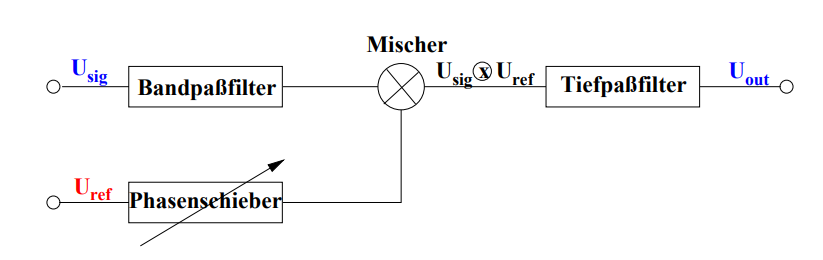
\includegraphics[width=\textwidth]{bilder/theo1.png}
    \caption{Schematische Darstellung der Funktionsweise eines Lock-In-Verstärkers.} 
    \label{fig:theo1}
\end{figure}
Dies lässt sich gut an einem Beispiel nachvollziehen. Wenn die Signalspannung sinusförmig, also die Spannung
\begin{equation*}
    U_{\text{s}} = U_0 \text{sin}(\omega t),
\end{equation*}
mit der Frequenz $\omega$ besitzt, dann lässt sich diese beispielweise durch eine Rechteckfunktion mit gleicher Frequenz modulieren. Die Rechteckfunktion lässt sich durch
die ungeraden Koeffizienten einer Fourierreihe darstellen
\begin{equation*}
    U_{\text{ref}} = \frac{4}{\pi}\left( \text{sin}(\omega t) + \frac{1}{3}  \text{sin}(3\omega t) + \frac{1}{5}  \text{sin}(5\omega t) + ...\right).
\end{equation*}
Diese Referenzspannung lässt sich nun mit der Signalspannung multiplizieren und es ergibt sich
\begin{equation*}
    U_{\text{mod}} = U_0 \frac{2}{\pi}\left(1- \frac{2}{3} \text{cos}(2\omega t) - \frac{2}{15}  \text{cos}(4\omega t) - \frac{2}{35}  \text{sin}(6\omega t) + ...\right).
\end{equation*}
In diesem Term sind die Oberwellen, also die Wellen mit $n \cdot \omega \quad | n \in \mathbb{N}\backslash\{1\}$ enthalten. Durch den Tiefpass werden diese unterdrückt und es ergibt 
sich eine Gleichspannung proportional zur Signalspannung. Allgemein kann es allerdings eine wie zuvor erwähnte Phasenverschiebung geben, womit folgender Zusammenhang gilt.
\begin{equation}
    U_{\text{out}} =\frac{2}{\pi}U_{0} \text{cos}(\phi).
\end{equation}

Die einzelnen Filter- und Modifikationsschritte sind in der Abbildung \ref{fig:theo2} für eine sinusförmige Signalspannung dargestellt.

\begin{figure}
    \centering
    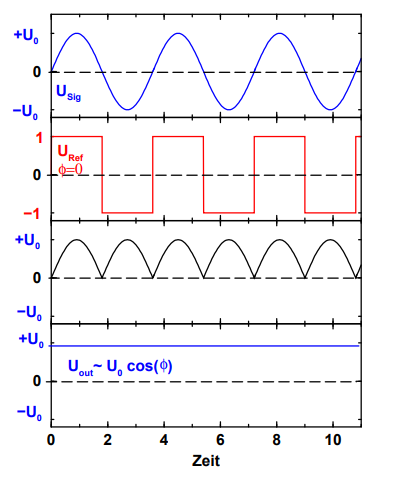
\includegraphics[width=0.54\textwidth]{bilder/theo2.png}
    \caption{Modifikationsschritte einer sinusförmigen Signalspannung mit Frequenz $\omega$.} 
    \label{fig:theo2}
\end{figure}